% !TeX spellcheck = en_US
\newpage
\section{SNMP}
The Simple Network Management Protocol allows the management of devices and services using a simple datagram service with a \textbf{client-server} architecture:
\begin{itemize}
	\item \textbf{Agent}: process continuously running on each managed node collecting information
	\item \textbf{Manager}: process running intermittently on a management workstation that requires information about the devices in the network
\end{itemize}
There may also be a \textbf{proxy agent} that integrates non-SNMP capable systems
\subsection{Motivation}
If we have problems in the network we need a \textbf{management tool} to be able to correctly identify them and their causes. In particular the tool needs to manage:
\begin{itemize}
	\item \textbf{Performance}: measure and analyze network performance to provide good network service
	\item \textbf{Configuration}: monitor or modify configuration settings or HW or SW elements
	\item \textbf{Accounting}: measure network utilization parameters per user or group of users
	\item \textbf{Fault}: detect, log, notify users and automatically fix problems while running
	\item \textbf{Security}: control access to network resources according to local guidelines to avoid sabotage and unauthorized access to sensitive information
\end{itemize}

\begin{observation}
	It should be achieved \textbf{remotely} over the existing network, meaning a protocol above IP.
\end{observation}

\subsubsection{Goals}
The main goals of network management are:
\begin{itemize}
	\item \textbf{Monitoring} HW equipment
	\item \textbf{Statistics} of network usage
	\item Remote \textbf{diagnostics}
	\item \textbf{Protected} and \textbf{safe} networking
	\item \textbf{Efficient} internetworking
	\item Simple model of \textbf{network status}
	\item Gather data for \textbf{network planning}
\end{itemize}

\subsection{Overview}
A network management framework is based on three building blocks:
\begin{itemize}
	\item \textbf{SNMP}: defines \textbf{format of messages} exchanged by management systems and agents and \textbf{basic operations}
	\item \textbf{SMI}: Structure of Management Information specifies how the monitored information is structured, defining the objects that SNMP protocol accesses over the network
	\item \textbf{MIB}: Management Information Base describes the concrete managed objects and is an open concept for data storage. It may be public (RFC) or proprietary.
\end{itemize}

\subsubsection{History}
There have been three major versions of SNMP during history:
\begin{itemize}
	\item \textbf{SNMPv1}, 1998, was designed originally as an interim solution but became the standard. It had very weak security model with complex bulk requests but was simpler than CMIS/CMIP
	\item \textbf{SNMPv2}, which was then split in
	\begin{itemize}
		\item \textit{SNMPv2u}: user-based security
		\item \textit{SNMPv2*}: user-based security and additional features
		\item \textit{SNMPv2c}: without security but with \textit{GetBulk} operation
	\end{itemize}
	\item \textbf{SNMPv3}, the current one, that provides an advanced security model: now each message has security parameters, integrity and authentication.
\end{itemize}

\subsection{Managed objects}
An \textit{agent} monitors the network resources that are abstracted as \textbf{managed objects}. Each one has a \textbf{unique ID} and a \textbf{name} and models various property of the resource. Its standard components are:
\begin{itemize}
	\item \textbf{Common prefix} + \textbf{Unique name}: e.g. \textit{iso.org.dod.internet.mgmt.mib.system.sysDescr}
	\item \textbf{Syntax}: simple data types \textit{integer}, \textit{string} and \textit{array}
	\item \textbf{Access rights}: \textit{read-only} or \textit{read-write}
	\item \textbf{Status}: \textit{mandatory} or \textit{optional}
\end{itemize}

\begin{wrapfigure}[7]{r}{3cm}
	\vspace{-1.5cm}
	\begin{center}
		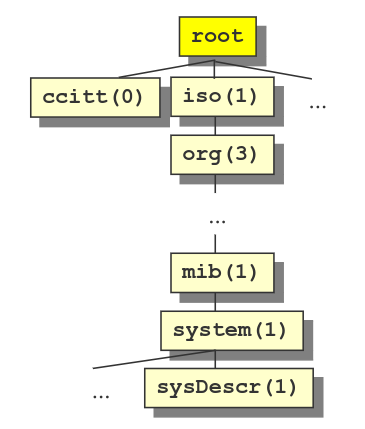
\includegraphics[width=3cm]{objs}
	\end{center}
\end{wrapfigure}
\paragraph{MIB}
The Management Information Base is a distributed virtual database that hosts the collection of managed objects that belong to the same context. It defines the capabilities of the device that can be managed.\\
In particular \textbf{MIB-2} defines the generics for all manageable internet devices. Its prefix is \textit{iso(1).org(3).dod(6).internet(1).mgmt(2).mib2(1)}. Some examples are \textit{batteryAgingNotification} with OID \textit{1.3.6.1.2.1.233.0.5} and \textit{sysLocation} with \textit{1.3.6.1.2.1.1.6}.\\
Another specific MIB is \textbf{RMON} for Remote Monitoring, it has more advanced functions such as gathering of statistics, alarms, events, on-board evaluations.
\paragraph{MIT}
Each managed object has a unique position in the Management Information Tree, thus providing a unique reference.

\begin{center}
	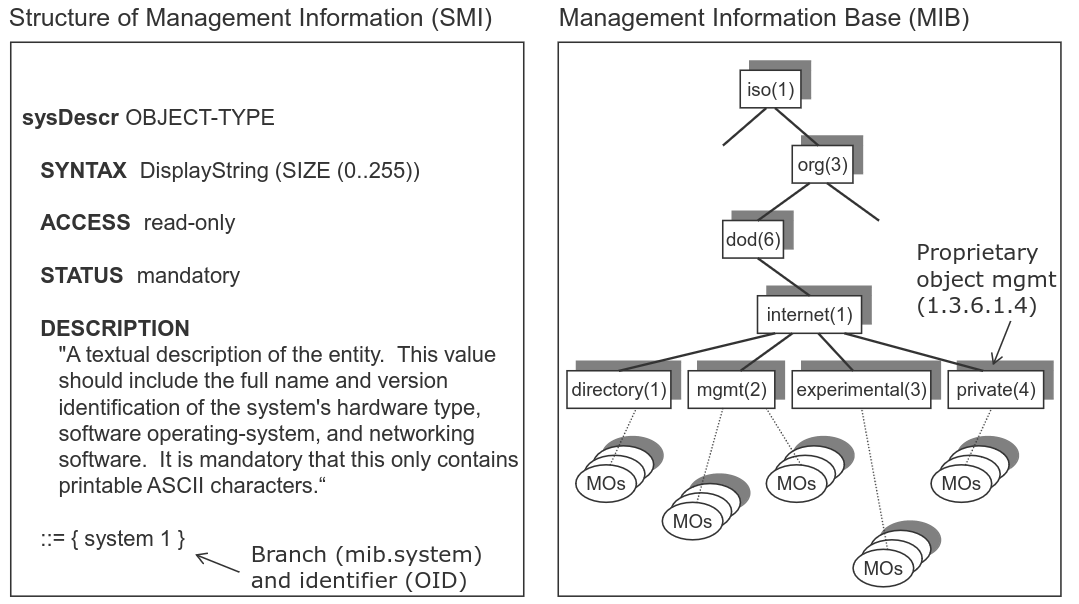
\includegraphics[scale=0.35]{mibsmi}
\end{center}

\subsubsection{Encoding}
Since different systems use different data representation, it's necessary to recode data while maintaining its meaning. To do that the message is first composed in ASN.1 syntax and then transferred using BER.
\paragraph{ASN.1}
Abstract Syntax Notation One is an ISO standardized language for representation-independent specification of data types. It's used in SNMP to describe managed objects. It consists of:
\begin{itemize}
	\item \textbf{Elementary} types, such as \textit{boolean}, \textit{integer}, \textit{bitstring}, $\ldots$
	\item \textbf{Structured} types:
	\begin{itemize}
		\item \textbf{Sequence}: ordered list of data types
		\item \textbf{Set}: unordered set of data types
		\item \textbf{Sequence Of}: like \textit{array} in C
		\item \textbf{Set Of}: unordered set of elements from the same data type
		\item \textbf{Choice}: like \textit{union} in C
	\end{itemize}
\end{itemize}
\begin{example}
	Some types defined by ASN.1:
	\begin{lstlisting}
		- INTEGER
			- signed 32-bit int
		- OCTET STRING
		- OBJECT IDENTIFIER (OID)
	\end{lstlisting}
	and some defined by SMI:
	\begin{lstlisting}
		- IpAddress
			- OCTET STRING of size 4, in network byte order
		- Counter
			- unsigned 32-bit int (rolls over)
		- Gauge
			- unsigned 32-bit int (will top out and stay there)
		- TimeTicks
			- unsigned 32-bit int (rolls over after 497 days)
		- Opaque
			- used to create new data types not in SNMPv1
		- DateAndTime, DisplayString, MacAddress, PhysAddress, TimeInterval, TimeStamp, TruthValue, VariablePointer
			- textual conventions used as types
	\end{lstlisting}
\end{example}

\paragraph{BER}
ASN.1 content is then converted into smaller binary data that follows the Basic Encoding Rules, like source code is converted to machine code.
\begin{center}
	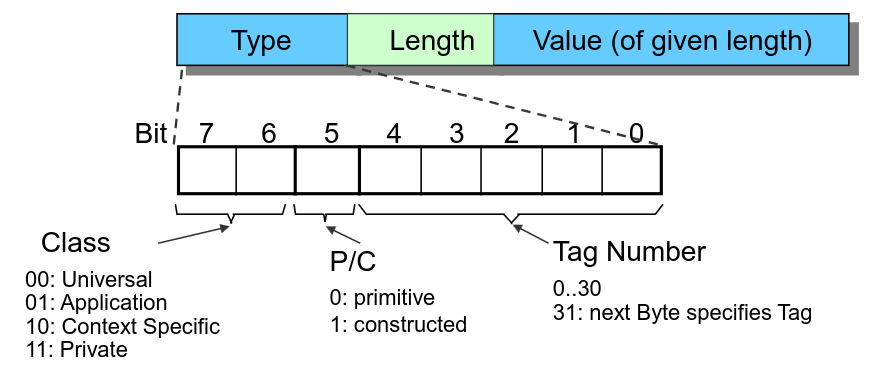
\includegraphics[scale=0.4]{ber}
\end{center}

\subsection{Operations}
SNMP has five main operations:
\begin{itemize}
	\item \textbf{GetRequest}, \textbf{GetNextRequest}, \textbf{SetRequest} and \textbf{GetResponse} that are initiated by the SNMP manager
	\item \textbf{Trap} that allows an agent to push information to the manager
	\item \textbf{GetBulkRequest} is a series of \textit{GetNextRequest}
\end{itemize}
\begin{center}
	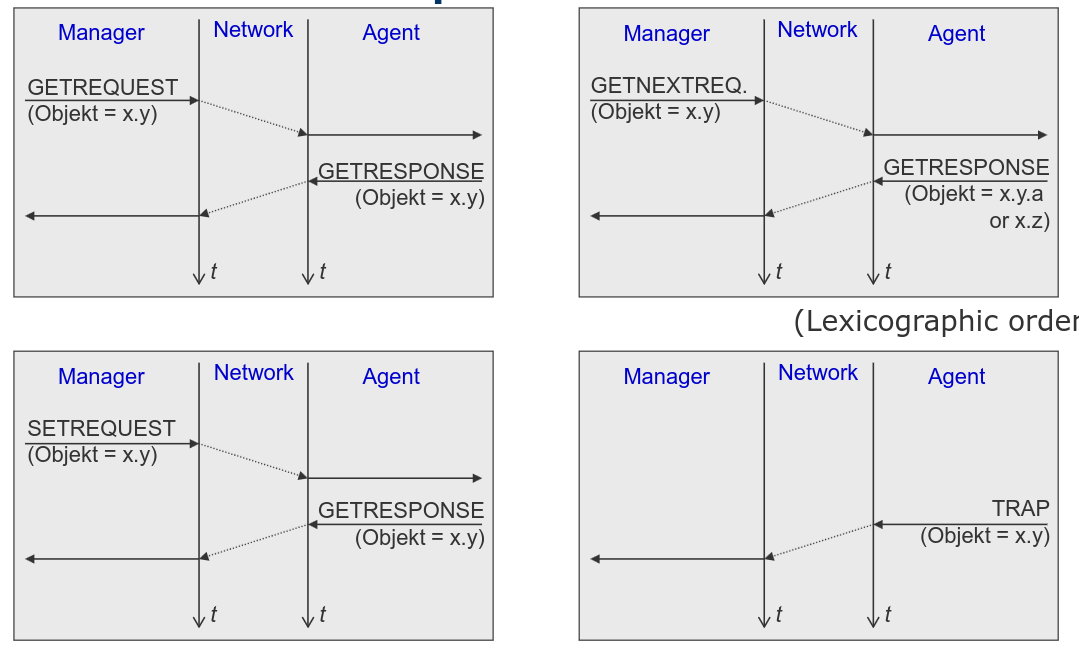
\includegraphics[scale=0.4]{ops}
\end{center}
SNMP works on a well-known UDP port: 161 for everything except of \textit{Trap} that is on 162.

\subsubsection{Packet format}
\begin{wraptable}[10]{r}{4cm}
	\vspace{5.7cm}
	\scalebox{1}{
		\begin{tabular}{c|c}
			0 & noError \\
			1 & tooBig \\
			2 & noSuchName \\
			3 & badValue \\
			4 & readOnly \\
			5 & genErr
		\end{tabular}
	}
\end{wraptable}
The packet is divided in:
\begin{center}
	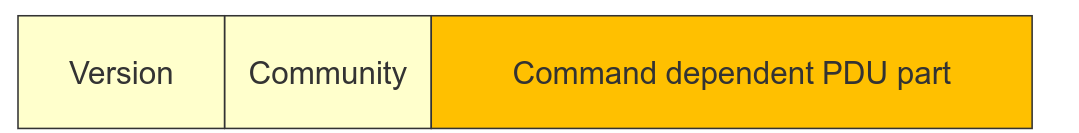
\includegraphics[scale=0.25]{packet1}
\end{center}
\begin{itemize}
	\item \textbf{Version}: version number of SNMP
	\item \textbf{Community}: string used for authentication, transmitted in plain text
	\item Command dependent\textbf{PDU}:
	\begin{center}
		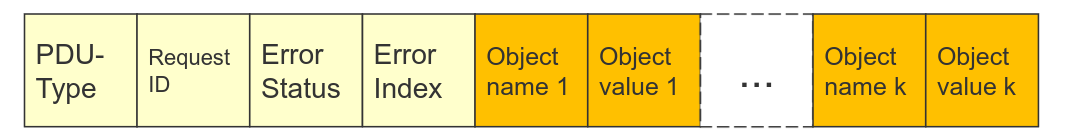
\includegraphics[scale=0.25]{packet2}
	\end{center}
	\begin{itemize}
		\item \textbf{PDU-Type}
		\item \textbf{Request Id}: identification of pending request
		\item \textbf{Error Status}, based on the result of the query
		\item \textbf{Error Index}: reference to the variable binding pair that caused the failure
		\item Variable length list of pairs of (Object Name, Object Value)
	\end{itemize}
\end{itemize}

\subsection{Tools}
There are different tools:
\begin{itemize}
	\item \textbf{Command line} like \textit{snmpget}, \textit{snmpnext}, etc that allows the generation and decoding of SNMP data units and sometimes also support for MIB files
	\item \textbf{MIB Browser}
	\item \textbf{Management Platforms} like \textit{CiscoWorks} and \textbf{Nagios} (open source)
\end{itemize}
All of the tools need to do the \textbf{discovery} and \textbf{polling} of the network topology through ICMP, SNMP and HTTP, among diffent devices with common interfaces but also vendor specific functionalities.

\subsection{NETCONF}
SNMP is used for monitoring only and therefore a tool for configuration is needed. NETCONF is based on XML and messages are exchanged through a secure transport protocol. The included operations are:
\begin{itemize}
	\item \textbf{get}: retrieve running configuration and device state information
	\item \textbf{get-config}: retrieve all or of a specified configuration datastore
	\item \textbf{edit-config}: edit a configuration datastore by creating, deleting, merging or replacing content
	\item \textbf{copy-config}: copy an entire configuration datastore to another configuration datastore
	\item \textbf{delete-config}: delete a configuration datastore
	\item \textbf{lock}: lock an entire configuration datastore of a device
	\item \textbf{unlock}: release a configuration datastore lock previously obtained with the \textit{lock} operation
	\item \textbf{close-session}: request graceful termination of a NETCONF session
	\item \textbf{kill-session}: force the termination of a NETCONF session 
\end{itemize}

An extension of NETCONF is \textbf{RESTCONF}, which allows accessing data defined in \textbf{YANG}. YANG (Yet Another Next Generation) is a data modeling language for the definition of the data. It can be used for configuration data, status of devices, events or notification. It's protocol independent but can be converted into XML or JSON. It's \textbf{modular} and represents data structures as XML tree, with many data types.
\subsubsection{NETCONF vs SNMP}
Let's analyze the main differences:
\begin{itemize}
	\item \textbf{Security}: NETCONF offers more granular and flexible access control mechanism, it runs over SSH or TLS (RESTCONF on HTTPS), while SNMP lacks proper encryption and authentication
	\item \textbf{Structure}: NETCONF uses structured data models to define the configuration and operational state of network devices, a clear and standardized way that reduces misconfigurations. On the other hand, SNMP is less structured and less intuitive (tree structure), often requiring complex OIDs and more prone to errors
	\item \textbf{Functionality}: SNMP can only retrieve device data while NETCONF can also modify or replace configurations
\end{itemize}